\pagebreak
\section{Teorema de la incompletitud matemática de Gödel}

\begin{wrapfigure}{l}{0.4\textwidth}
    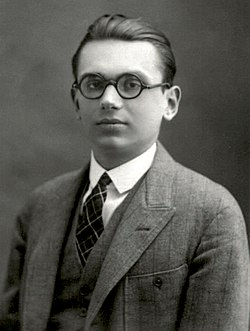
\includegraphics[width=5cm]{figures/Kurt_Godel.jpg}
    \caption{Gödel como estudiante a los 19 años de edad, 5 años antes de la 
    demostración de los teoremas.}
\end{wrapfigure}

Gödel, nacido el 28 de abril de 1906 en Brno (hoy parte de la República Checa),
demostró como parte de su tesis doctoral, en 1929, el primer teorema de
incompletitud, que afirma que todo sistema axiomático coherente que englobe las
propiedades aritméticas básicas de los números naturales padece una dicotomía
\footnote{División de un concepto o una materia teórica en dos aspectos,
especialmente cuando son opuestos o están muy diferenciados entre sí.}
fundamental: o bien no se puede implementar en un algoritmo, o bien los axiomas
no son capaces de determinar la veracidad de todos los enunciados posibles.
Gödel demostró que en todo “universo matemático” imaginable habrá propiedades
que no podemos demostrar.

Los enunciados matemáticos indecidibles son imposibles de evitar. Un ejemplo es
la hipótesis del continuo, que afirma que todo subconjunto infinito de los
números reales se puede identificar con los números naturales o con los reales.
Otro ejemplo es el axioma de elección, que afirma que dada una colección de
cajas (o conjuntos) no vacías, es posible escoger un elemento de cada caja.
Puede resultar sorprendente que este axioma sea problemático, sobre todo si sólo
pensamos en un número finito de cajas. Sin embargo, en un contexto infinito,
tiene consecuencias inesperadas: Stefan Banach y Alfred Tarski demostraron
partiendo de dicho axioma que se puede descomponer una bola de madera maciza en
un número finito de piezas, las cuales, recolocadas de cierta manera, dan como
resultado dos bolas del mismo volumen.

El teorema de Gödel o teorema de incompletitud limita las posibilidades de las
matemáticas de demostrar fórmulas a través de la deducción. Dibuja el límite a
lo que es posible conocer a través de la lógica formal tal y como se plantea en
física y otras disciplinas.  Muy resumidamente hablando, el teorema de Gödel
viene a decir que «no se puede demostrar cualquier fórmula matemática, aunque
sea verdadera».

La demostración del teorema de incompletitud se apoya en dos ideas claves: por
un lado, Gödel tuvo la destreza de codificar frases y enunciados a través de
números. Al hablar de números, ahora hablamos también de enunciados. Por otro
lado, utilizó un argumento diagonal semejante al que usó Georg Cantor para
demostrar que, pese a que hay tantos números racionales como naturales, hay
muchos más números reales que naturales.

A raíz de los trabajos de Gödel se consolidaron diversas disciplinas dentro de
la lógica matemática: por un lado, la teoría de conjuntos como paradigma de un
formalismo autosuficiente, la teoría de la recursión y de la demostración, con
un enfoque sintáctico y algorítmico, así como la teoría de modelos, en la que
trabajamos los autores de este artículo, que se concentra en las propiedades
semánticas de los objetos matemáticos.

David Hilbert (1862-1943) se preguntaba si las matemáticas eran completas,
consitentes y decidibles.

El teorema de la incompletitud de Gödel significa que la verdad y la
demostrabilidad no son lo mismo en absoluto. Hilbert estaba equivocado. Siempre
habrá afirmaciones verdaderas sobre la matemática que no podamos demostrar.

También demostro que la matemática no es consistente (libre de contradicciones),
ya que cualquier sistema formal consistente de la matemática es incapaz de
probar su propia consistencia (paradojas de autoreferencia). Así que tomando
ambos teoremas de la incompletitud de Gödel, estos dicen que lo mejor a lo que
podemos aspirar es a un sistema consistente pero incompleto de la matemática.
Pero un sistema coo ese no puede probar su propia consistencia, por lo que
algunas contradicciones podrían surgir en el futuro revelando que el sistema en
el que se trabaja ha sido inconsistente todo el tiempo.

% Eso nos deja la tercera y última pregunta de Hilbert; ¿es la matemática
% decidible?, ¿Hay algún algoritmo que pueda siempre determinar si una afirmación
% surge de los axiomas?.


% doxygen

